\documentclass[12pt,a4paper]{article}
\usepackage{geometry}
\geometry{left=2.5cm,right=2.5cm,top=2.0cm,bottom=2.5cm}
\usepackage[english]{babel}
\usepackage{amsmath,amsthm}
\usepackage{amsfonts}
\usepackage[longend,ruled,linesnumbered]{algorithm2e}
\usepackage{siunitx}
\usepackage{fancyhdr}
\usepackage{ctex}
\usepackage{array}
\usepackage{listings}
\usepackage{color}
\usepackage{graphicx}
\usepackage{float}
\usepackage{caption}
\usepackage{longtable}
\begin{document}
    \title{\heiti{《机器学习》课程第 {$1$} 次作业}}
    \date{}
    \author{姓名:\underline{刘哲}~~~~~~学号:\underline{2022103691}~~~~~~}
    \maketitle
    \section{\heiti{生鲜销量}}
    \vspace{10pt}
    \subsubsection*{A}
    生鲜销量数据的时间序列图如下:
    \begin{figure}[H]
        \centering
        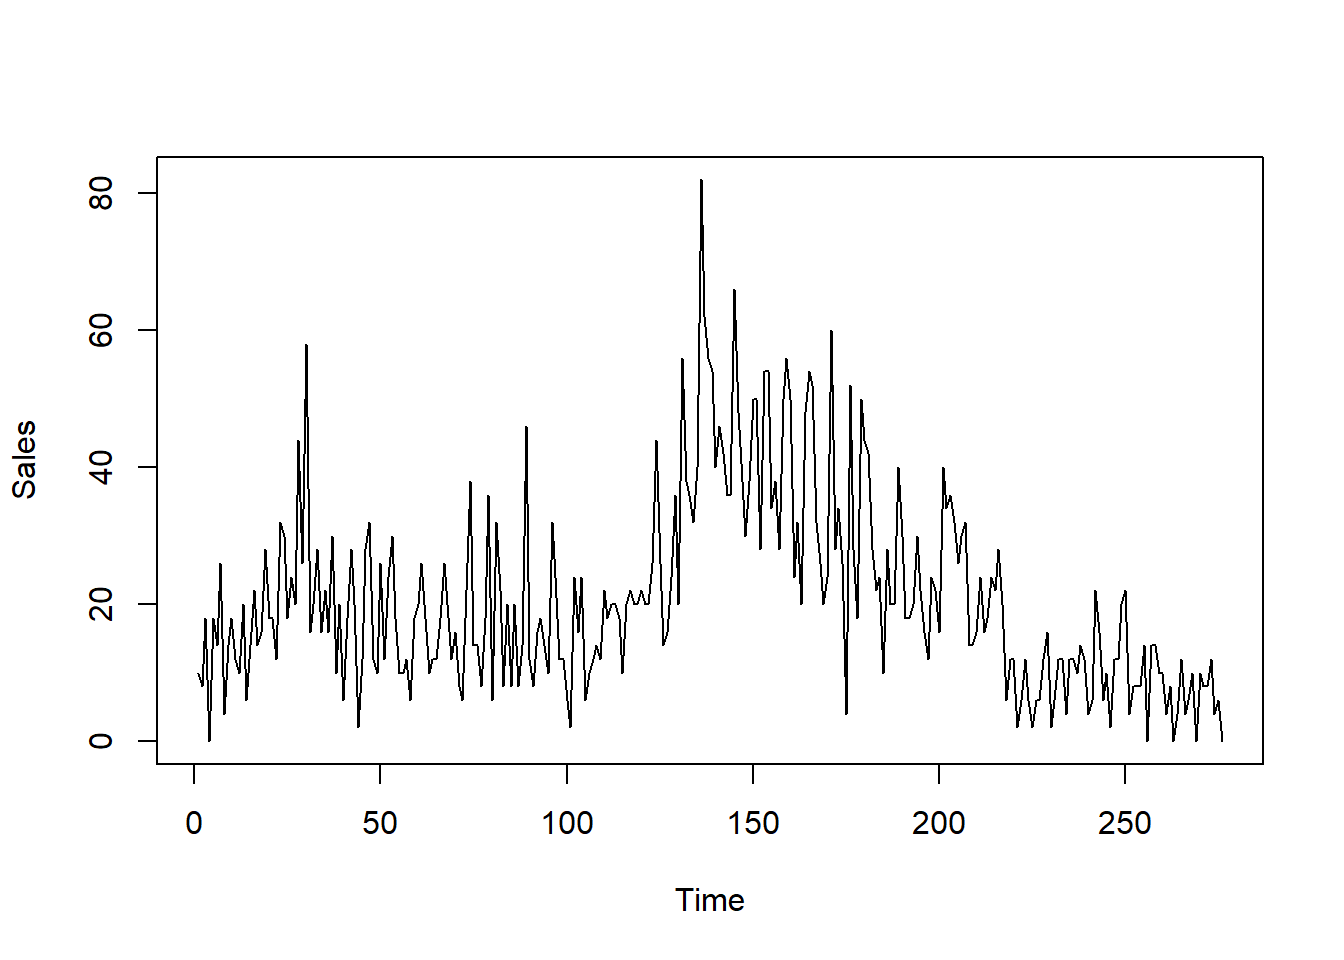
\includegraphics[scale=0.8]{FreshTS.png}
        \caption*{生鲜日销量序列}
    \end{figure}
    如图所示,序列有比较明显的先上升再下降的趋势,因此采用以下3种模型拟合数据:
    \begin{itemize}
        \item ARIMA模型:建立ARIMA模型需要假设时间序列数据差分平稳,同时不能为白噪声数据,否则没有分析价值。
        模型表示为$x_t-x_{t-1}=\varepsilon_t-\theta\varepsilon_{t-1}$,其中$\varepsilon_t\sim N(0,\sigma_1^2)$。
        \item 残差自回归模型:因为数据有明显的先升后降趋势,可以先通过确定性因素分解方法提取序列中主要的确定性信息,假设残差项之间具有自相关关系,并拟合残差自回归模型提取。
        模型表示为$x_t=c+bt+at^2+\varepsilon_t$,$\varepsilon_t=\theta_1\varepsilon_{t-1}+\theta_5\varepsilon_{t-5}+e_t$,其中$e_t\sim N(0,\sigma_2^2)$。
        \item 线性回归模型:建立线性回归模型需要假设残差项满足Gauss假定。
        模型表示为$x_t=a_0+a_1t+a_2t^2+a_3t^3+a_4t^4+a_5t^5+\varepsilon_t$,其中$\varepsilon_t\sim N(0,\sigma_3^2)$。
    \end{itemize}
    \subsubsection*{B}
    利用训练集数据拟合模型,得到3个模型的参数,则拟合模型分别为:
    \begin{itemize}
        \item ARIMA(0,1,1):$x_t-x_{t-1}=\varepsilon_t+0.7998\varepsilon_{t-1}$,其中$\varepsilon_t\sim N(0,103.6)$。
        \item 残差自回归模型:$x_t=7.5760+0.3261t-\num{1.2416e-3}t^2+\varepsilon_t$,$\varepsilon_t=0.3570\varepsilon_{t-1}+0.3358\varepsilon_{t-5}+e_t$,其中$e_t\sim N(0,101)$。
        \item 线性回归模型:$x_t=11.30+0.7897t-\num{2.476e-02}t^2+\num{2.935e-04}t^3-\num{1.363e-06}t^4+\num{2.131e-09}t^5+\varepsilon_t$,其中$\varepsilon_t\sim N(0,116.4241)$。
    \end{itemize}
    \subsubsection*{C}
    经检验,拟合模型均显著,且模型参数均显著:
    \begin{itemize}
        \item ARIMA(0,1,1):Box检验的$p-value=0.2616$,表明ARIMA(0,1,1)模型的残差序列为白噪声序列,信息提取完全,拟合模型显著。
        参数$\theta$显著性t检验的$p-value=\num{6.5609e-68}$,表明模型参数显著。
        参数$\theta$为模型的移动平均系数,表示延期随机干扰项对当期销量的影响程度。
        \item 残差自回归模型:Box检验的$p-value=0.204$,表明残差自回归模型的残差序列为白噪声序列,信息提取完全,拟合模型显著。
        参数$\theta_1$和$\theta_5$显著性t检验的$p-value$分别为$\num{2.795988e-11}$和$\num{2.652622e-10}$,表明模型参数显著。
        参数$\theta_1$和$\theta_5$为残差自回归系数,表示销量残差序列的前后期自相关程度。
        \item 线性回归模型:F检验的$p-value<\num{2.2e-16}$,表明拟合模型显著。
        参数$a_0$、$a_1$、$a_2$、$a_3$、$a_4$和$a_5$显著性t检验的$p-value<0.01$,表明模型参数显著。
        参数$a_0$、$a_1$、$a_2$、$a_3$、$a_4$和$a_5$为回归系数,表示销量受时间变化的影响程度。
    \end{itemize}
    \subsubsection*{D}
    使用拟合模型对测试数据进行预测,计算MSE作为预测销量和实际销量的测试误差:
    \begin{itemize}
        \item ARIMA(0,1,1):固定第一期的时间序列值,根据模型表达式依次预测将来期的序列值,并将负数的预测值修改为0。测试误差为1311.623。
        \item 残差自回归模型:固定前五期的时间序列值,根据模型表达式依次预测将来期的序列值,并将负数的预测值修改为0。测试误差为7935.799。
        \item 线性回归模型:将时间t代入模型表达式,预测出对应的序列值。测试误差为7834.214。
    \end{itemize}
    \subsubsection*{E}
    各个模型的拟合序列图如下:
    \begin{figure}[H]
        \centering
        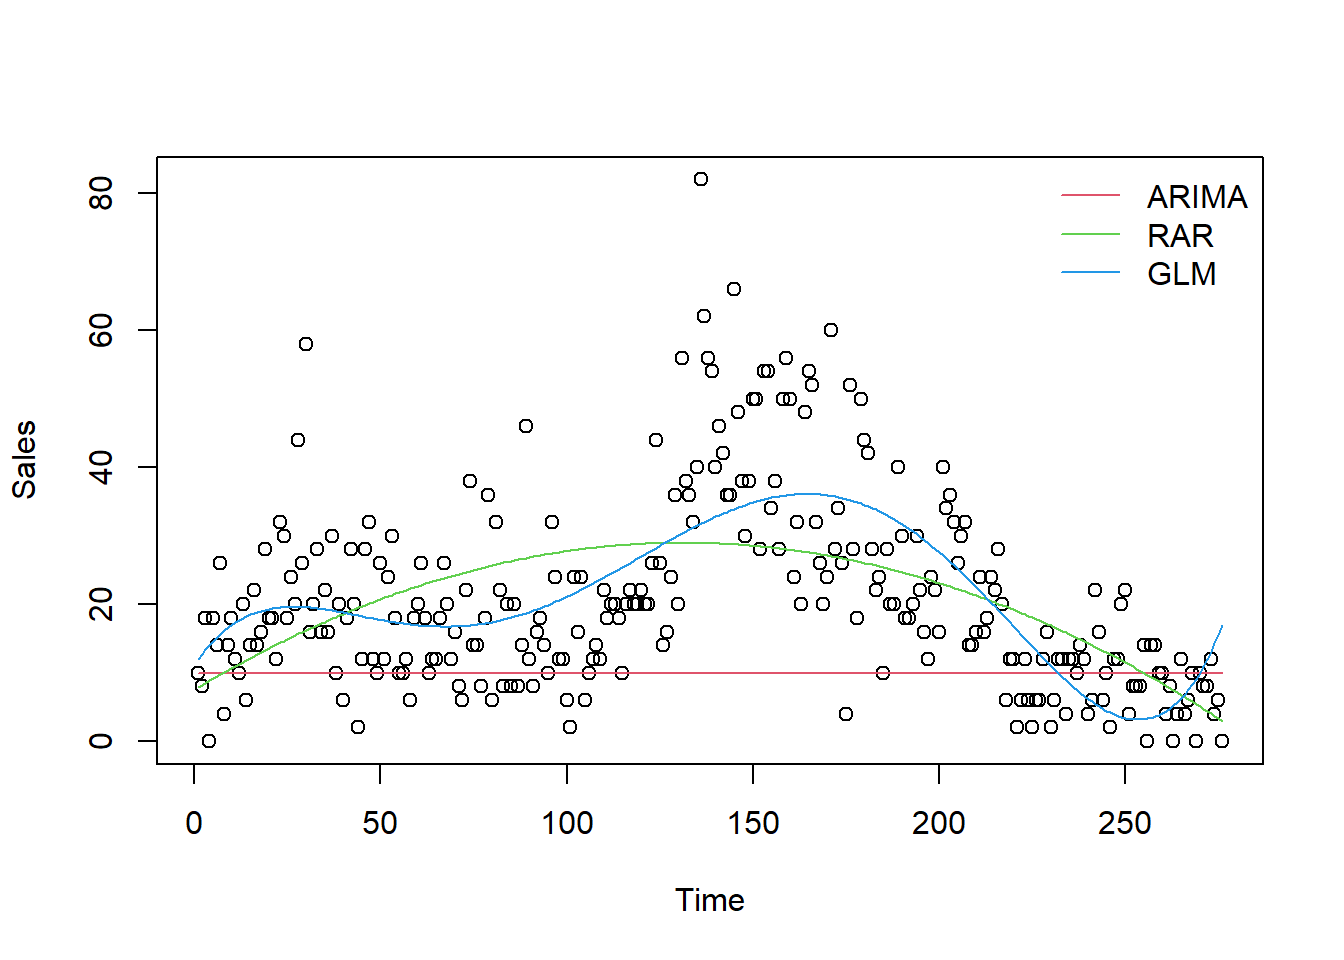
\includegraphics[scale=0.8]{FreshFitting.png}
        \caption*{拟合序列图}
    \end{figure}
    各个模型的MSE随模型柔性的变化图如下:
    \begin{figure}[H]
        \centering
        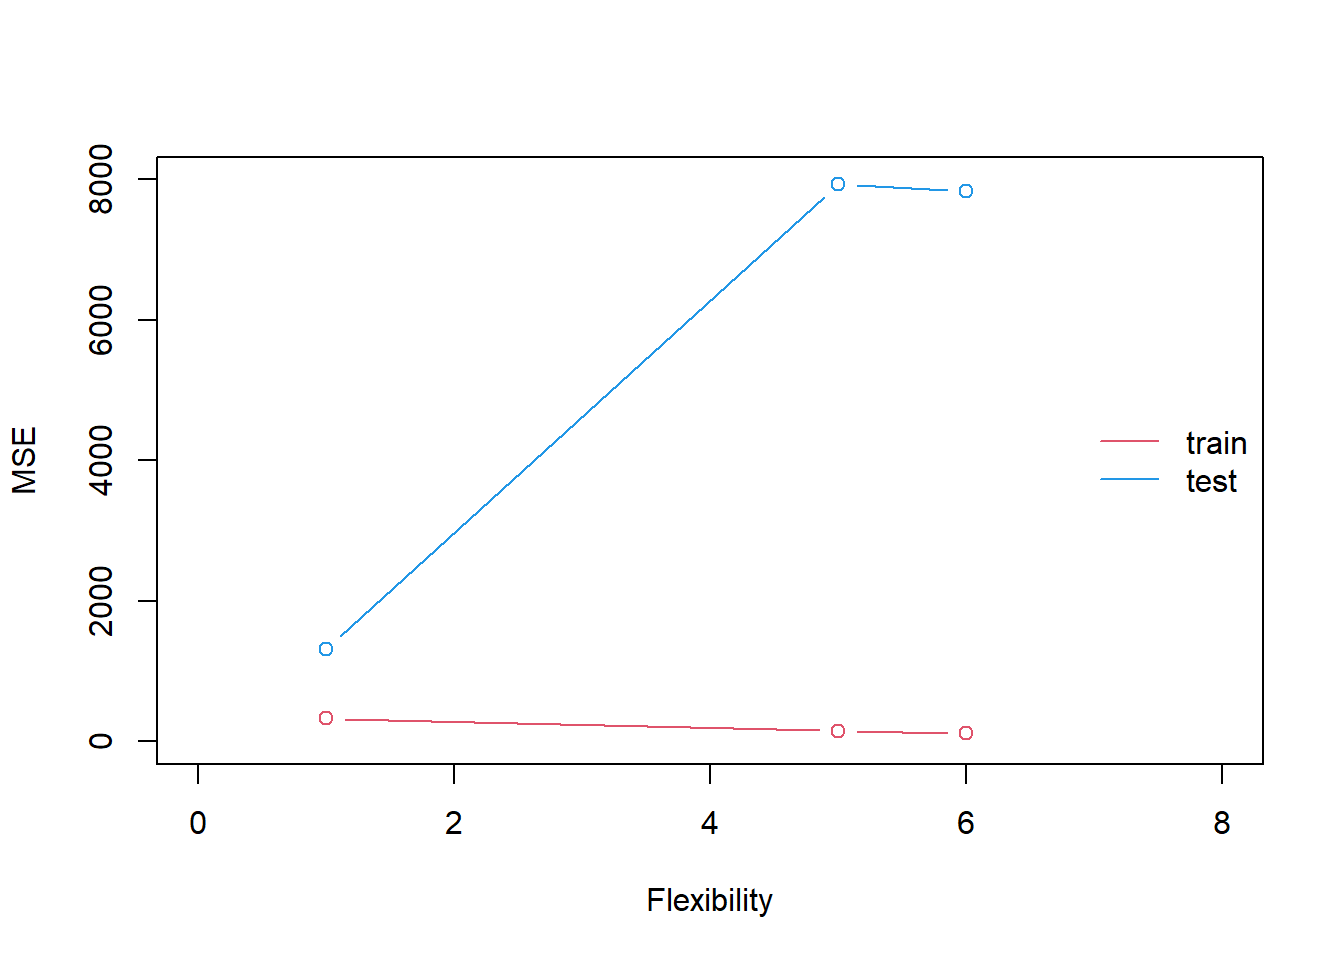
\includegraphics[scale=0.8]{FreshMSEFlexibility.png}
    \end{figure}
    如图所示,在训练数据上表现最好的是线性回归模型,表现最差的是ARIMA模型。
    但由于测试数据与训练数据的差别过于巨大,导致残差自回归模型和线性回归模型在测试集数据上的表现极差;
    虽然ARIMA模型柔性最低,训练误差最大,但在测试数据上有最好的表现。
    因此,对于该生鲜日销量数据,最适合的预测建模为ARIMA模型。
    \section{\heiti{墨迹鉴定}}
    \subsubsection*{A}
    通过比较逻辑回归、决策树、随机森林等分类模型的训练误差和预测误差,选择训练效果和预测效果最好的随机森林分类模型。\par
    模型的超参数会在很大程度上影响模型的预测效果。随机森林分类模型中有两个主要的超参数:构建决策树分支时抽取的变量个数(mtry)和随机森林中树的数量(ntree)。\par
    选择mtry范围为1$\sim$3(数据中共有3个变量),ntree范围为100$\sim$1000(间隔100),两两组合成30组超参数对,每组训练10个随机森林模型,比较各个模型的错误率。\par
    使用瓶装墨迹数据训练模型,测试数据错误率最低的10个模型的超参数如下:
    \begin{longtable}{c|c|c|c|c}
        \hline
        \textbf{iter} & \textbf{mtry} & \textbf{ntree} & \textbf{obb error} & \textbf{test error}\\
        \hline
        3 & 1 & 300 & 0.42 & 0.56\\
        \hline
        4 & 1 & 100 & 0.40 & 0.56\\
        \hline
        6 & 1 & 400 & 0.42 & 0.56\\
        \hline
        1 & 1 & 300 & 0.42 & 0.58\\
        \hline
        1 & 1 & 500 & 0.44 & 0.58\\
        \hline
        1 & 1 & 600 & 0.42 & 0.58\\
        \hline
        1 & 1 & 700 & 0.40 & 0.58\\
        \hline
        1 & 1 & 800 & 0.42 & 0.58\\
        \hline
        1 & 1 & 900 & 0.38 & 0.58\\
        \hline
        2 & 1 & 300 & 0.40 & 0.58\\
        \hline
    \end{longtable}
    因此,在使用瓶装墨迹数据训练模型时,设置$mtry=1$,$ntree=100$。\par
    使用简装墨迹数据训练模型,测试数据错误率最低的10个模型的超参数如下:
    \begin{longtable}{c|c|c|c|c}
        \hline
        \textbf{iter} & \textbf{mtry} & \textbf{ntree} & \textbf{obb error} & \textbf{test error}\\
        \hline
        1 & 2 & 100 & 0.32 & 0.72\\
        \hline
        7 & 3 & 200 & 0.28 & 0.74\\
        \hline
        1 & 3 & 100 & 0.28 & 0.76\\
        \hline
        2 & 2 & 200 & 0.30 & 0.76\\
        \hline
        2 & 3 & 100 & 0.26 & 0.76\\
        \hline
        3 & 3 & 100 & 0.30 & 0.76\\
        \hline
        4 & 3 & 200 & 0.28 & 0.76\\
        \hline
        4 & 3 & 900 & 0.28 & 0.76\\
        \hline
        5 & 3 & 100 & 0.30 & 0.76\\
        \hline
        5 & 3 & 300 & 0.30 & 0.76\\
        \hline
    \end{longtable}
    因此,在使用简装墨迹数据训练模型时,设置$mtry=2$,$ntree=100$。\par
    通过观察可以发现,瓶装墨迹模型的测试错误率明显小于简装墨迹模型的测试错误率,
    而简装墨迹模型的袋外错误率略小于瓶装墨迹模型的袋外错误率。
    原因可能是简装墨迹成分变异导致解释变量差异增大,更容易区分训练数据中的不同墨迹;
    但同时也因此增大了鉴定的难度,造成其在测试数据上的错误率更高。
    \subsubsection*{B}
    瓶装墨迹模型训练数据的混淆矩阵如下:
    \begin{longtable}{c|ccccc}
        \hline
        \textbf{ink} & \textbf{1} & \textbf{2} & \textbf{3} & \textbf{4} & \textbf{5}\\
        \hline
        \textbf{1} & 6 & 3 & 1 & 0 & 0\\
        \textbf{2} & 5 & 0 & 4 & 0 & 1\\
        \textbf{3} & 2 & 3 & 5 & 0 & 0\\
        \textbf{4} & 0 & 0 & 0 & 9 & 1\\
        \textbf{5} & 1 & 0 & 0 & 1 & 8\\
        \hline
    \end{longtable}
    简装墨迹模型训练数据的混淆矩阵如下:
    \begin{longtable}{c|ccccc}
        \hline
        \textbf{ink} & \textbf{1} & \textbf{2} & \textbf{3} & \textbf{4} & \textbf{5}\\
        \hline
        \textbf{1} & 7 & 2 & 1 & 0 & 0\\
        \textbf{2} & 3 & 2 & 4 & 0 & 1\\
        \textbf{3} & 1 & 3 & 6 & 0 & 0\\
        \textbf{4} & 0 & 0 & 0 & 9 & 1\\
        \textbf{5} & 1 & 0 & 0 & 1 & 8\\
        \hline
    \end{longtable}
    由此可知,使用两种不同的训练数据建立的模型在第二种墨迹上的错误率都非常高,而在第四、五种墨迹上的错误率都比较低;
    同时瓶装墨迹模型的袋外错误率(44\%)略高于简装墨迹模型的袋外错误率(36\%)。
    \subsubsection*{C}
    瓶装墨迹模型测试数据的混淆矩阵如下:
    \begin{longtable}{c|ccccc}
        \hline
        \textbf{ink} & \textbf{1} & \textbf{2} & \textbf{3} & \textbf{4} & \textbf{5}\\
        \hline
        \textbf{1} & 9 & 0 & 0 & 1 & 0\\
        \textbf{2} & 4 & 3 & 3 & 0 & 0\\
        \textbf{3} & 0 & 8 & 2 & 0 & 0\\
        \textbf{4} & 0 & 0 & 2 & 0 & 8\\
        \textbf{5} & 0 & 0 & 3 & 0 & 7\\
        \hline
    \end{longtable}
    简装墨迹模型测试数据的混淆矩阵如下:
    \begin{longtable}{c|ccccc}
        \hline
        \textbf{ink} & \textbf{1} & \textbf{2} & \textbf{3} & \textbf{4} & \textbf{5}\\
        \hline
        \textbf{1} & 9 & 0 & 0 & 1 & 0\\
        \textbf{2} & 4 & 3 & 3 & 0 & 0\\
        \textbf{3} & 1 & 6 & 3 & 0 & 0\\
        \textbf{4} & 2 & 0 & 0 & 0 & 8\\
        \textbf{5} & 1 & 1 & 5 & 0 & 3\\
        \hline
    \end{longtable}
    由此可知,瓶装墨迹模型在第一、五种墨迹上的错误率都比较低,而在第二、三、四种墨迹上的错误率都比较高;
    简装墨迹模型在第一种墨迹上的错误率很低,在其他墨迹上的错误率都很高。
    同时瓶装墨迹模型的测试错误率(58\%)低于简装墨迹模型的测试错误率(64\%)。\par
    发生这种变化的原因可能是简装墨迹的成分变异既使得墨迹特征更加突出,又造成墨迹之间更难区分。
    因此,认为瓶装墨迹模型表现较好。\par
    瓶装墨迹模型的单一墨迹训练误差如下:
    \begin{longtable}{c|c}
        \hline
        \textbf{ink} & \textbf{class.error}\\
        \hline
        1 & 0.4\\
        2 & 1.0\\
        3 & 0.5\\
        4 & 0.1\\
        5 & 0.2\\
        \hline
    \end{longtable}
    瓶装墨迹模型的单一墨迹测试误差如下:
    \begin{longtable}{c|c}
        \hline
        \textbf{ink} & \textbf{class.error}\\
        \hline
        1 & 0.1\\
        2 & 0.7\\
        3 & 0.8\\
        4 & 1.0\\
        5 & 0.3\\
        \hline
    \end{longtable}
    \subsubsection*{D}
    瓶装墨迹模型中每一种墨迹的微训练误差如下:
    \begin{longtable}{c|c}
        \hline
        \textbf{ink} & \textbf{class.error}\\
        \hline
        1 & 0.1335\\
        2 & 0.1875\\
        3 & 0.1187\\
        4 & 0.0375\\
        5 & 0.0683\\
        \hline
    \end{longtable}
    瓶装墨迹模型中每一种墨迹的微测试误差如下:
    \begin{longtable}{c|c}
        \hline
        \textbf{ink} & \textbf{class.error}\\
        \hline
        1 & 0.1087\\
        2 & 0.2000\\
        3 & 0.1563\\
        4 & 0.1785\\
        5 & 0.1639\\
        \hline
    \end{longtable}
    \subsubsection*{E}
    瓶装墨迹模型的整体微训练误差为$0.1091$,整体微测试误差为$0.1889$。
    \subsubsection*{F}
    建立模型的目的是从化学成分$x$、$y$和$z$的比例结构中找出能区分出5种墨迹的特征,因此用于训练模型的数据应该能够比较稳定地表现出各种墨迹的化学结构特征。
    简装墨迹会加速墨迹的成分变异,无法保持一个比较稳定的化学成分结构,所以即使其模型训练误差较低,测试误差却非常高,不适合用于建立预测模型。
    而瓶装墨迹能够保持较为稳定的化学成分结构,训练出的模型会有更好的预测效果。
    \subsubsection*{G}
    \begin{figure}[H]
        \centering
        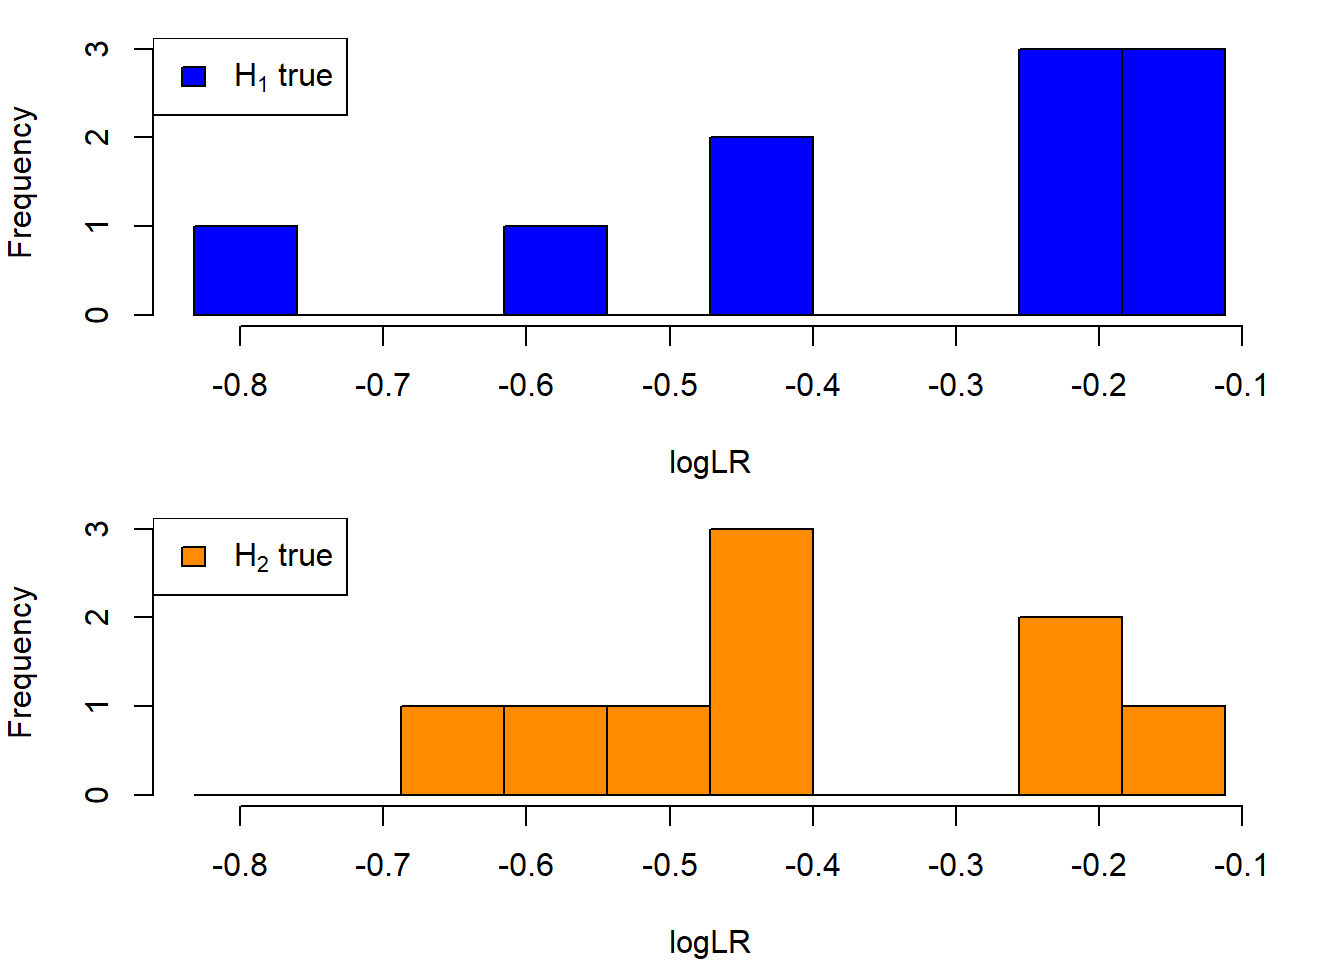
\includegraphics[scale=0.8]{InkHist1.png}
        \caption*{墨迹1的Histogram图}
    \end{figure}
    \begin{figure}[H]
        \centering
        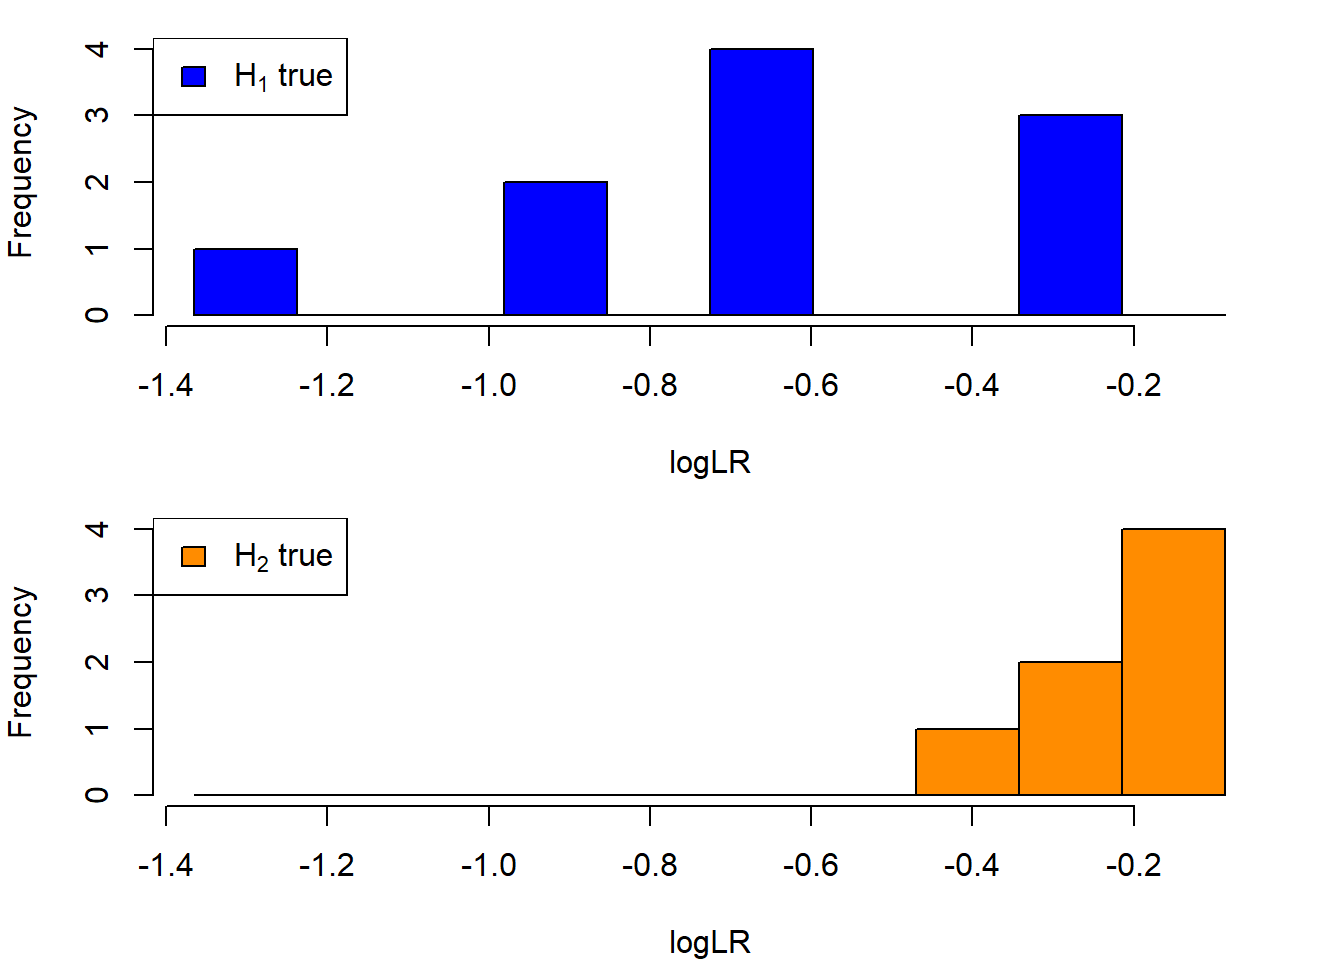
\includegraphics[scale=0.8]{InkHist2.png}
        \caption*{墨迹2的Histogram图}
    \end{figure}
    \begin{figure}[H]
        \centering
        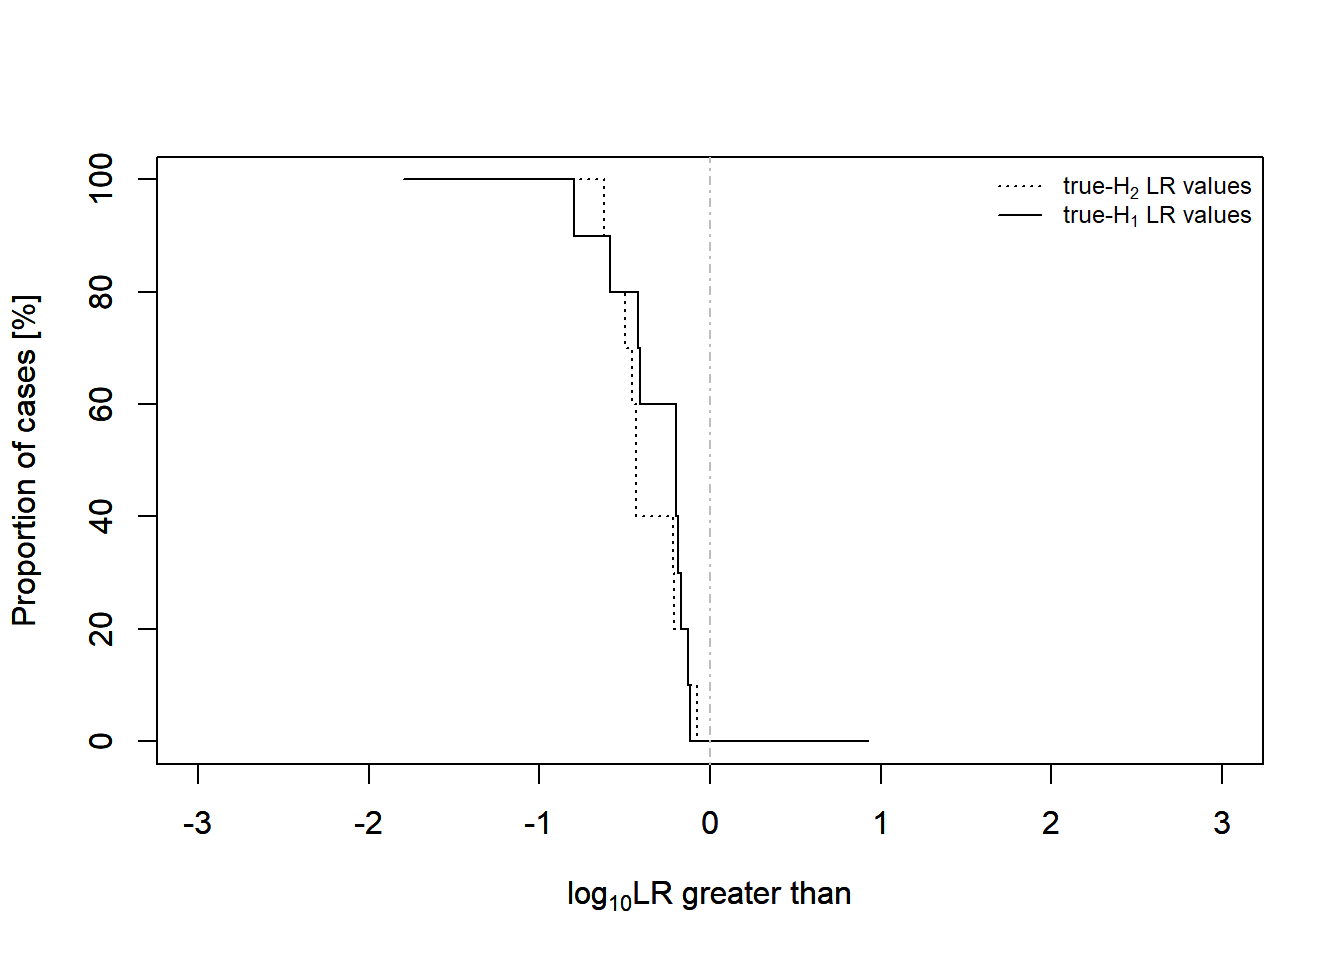
\includegraphics[scale=0.8]{InkTippett1.png}
        \caption*{墨迹1的Tippett图}
    \end{figure}
    \begin{figure}[H]
        \centering
        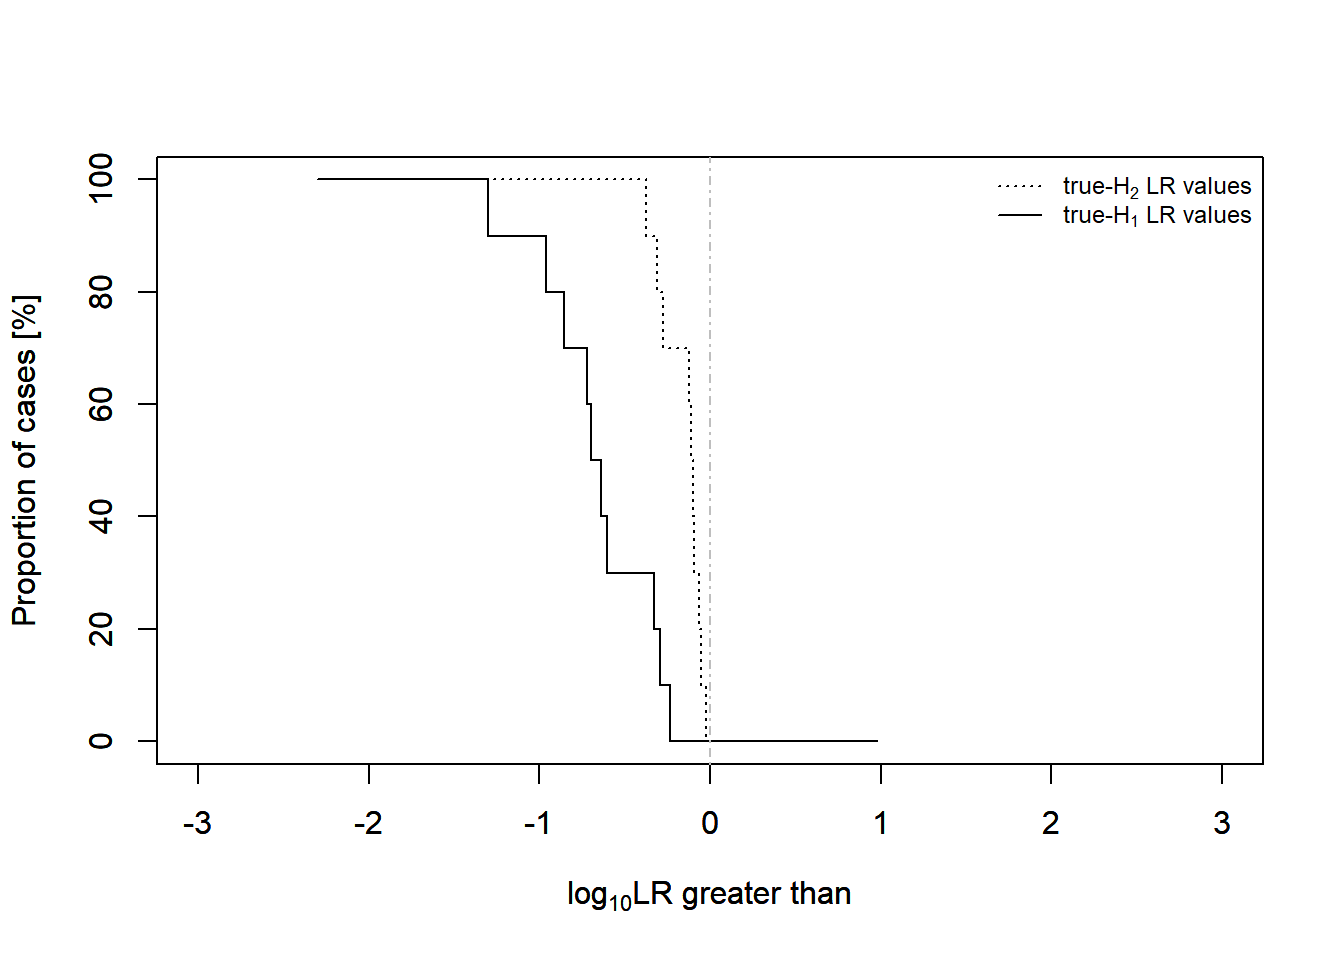
\includegraphics[scale=0.8]{InkTippett2.png}
        \caption*{墨迹2的Tippett图}
    \end{figure}
    \begin{figure}[H]
        \centering
        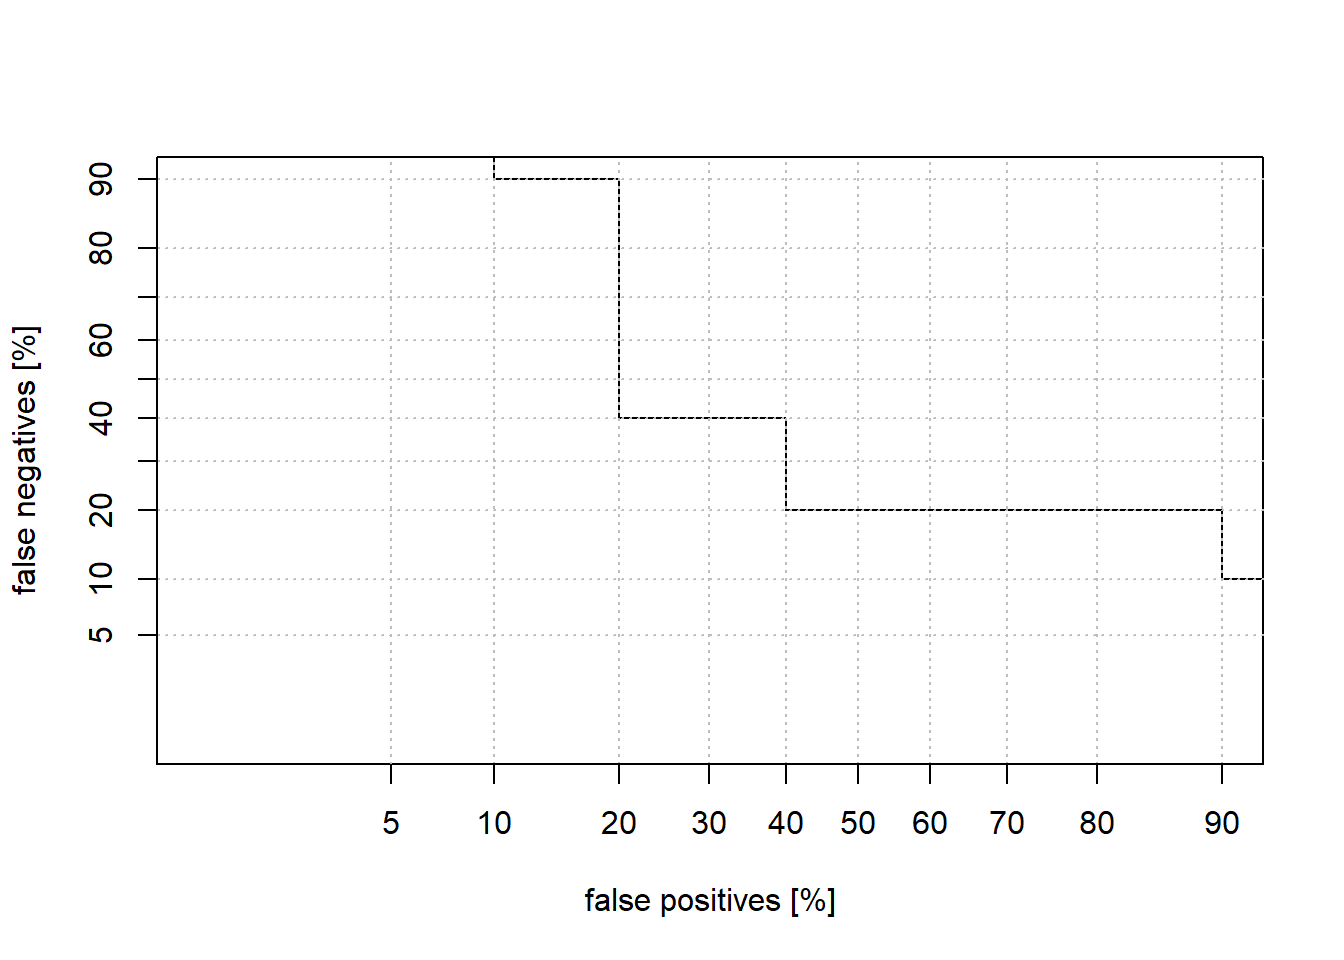
\includegraphics[scale=0.8]{InkDET1.png}
        \caption*{墨迹1的DET图}
    \end{figure}
    \begin{figure}[H]
        \centering
        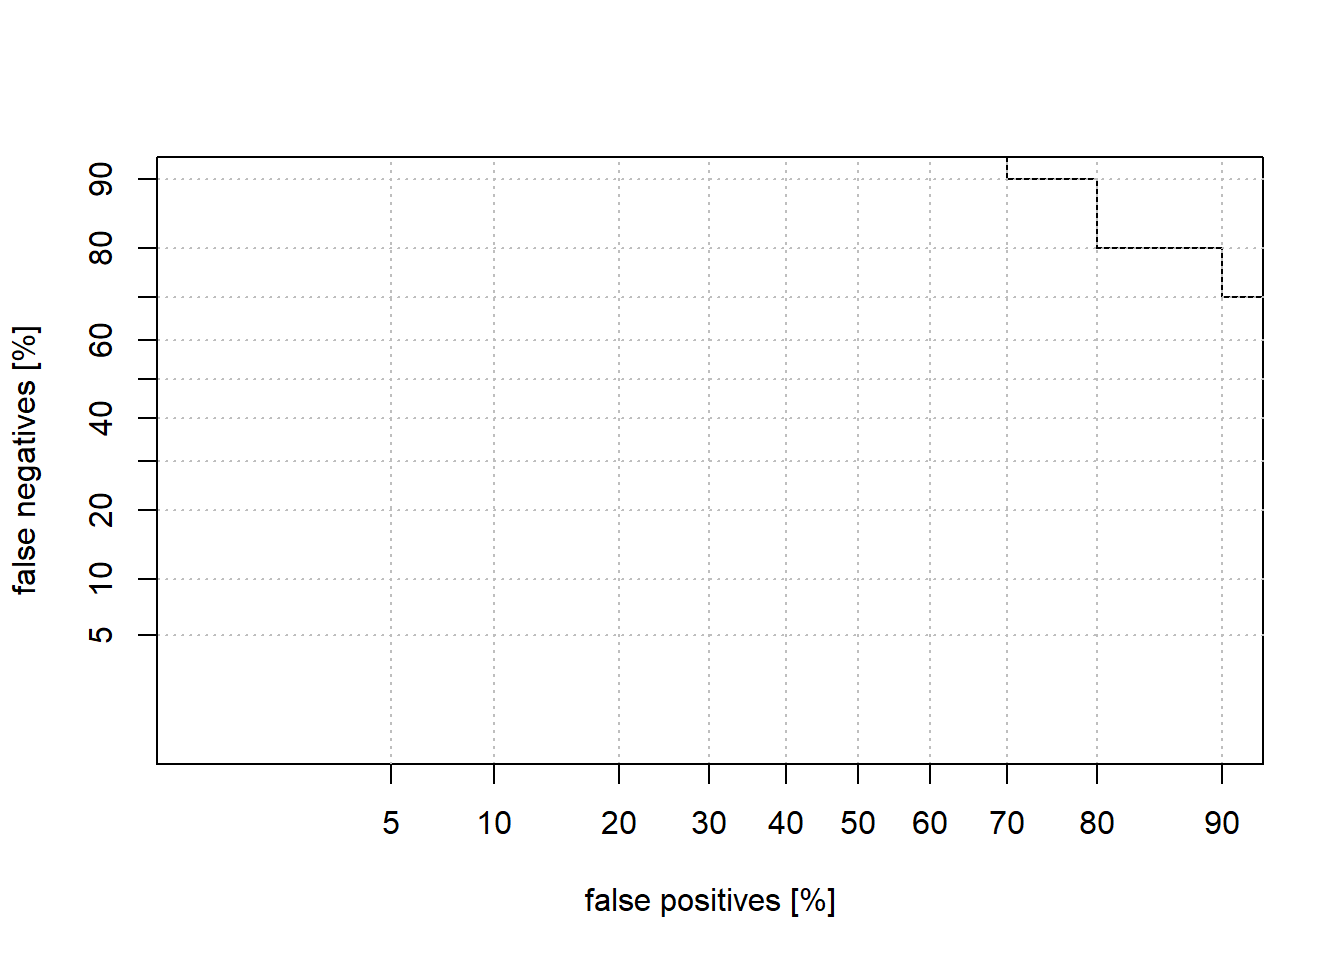
\includegraphics[scale=0.8]{InkDET2.png}
        \caption*{墨迹2的DET图}
    \end{figure}
    \begin{figure}[H]
        \centering
        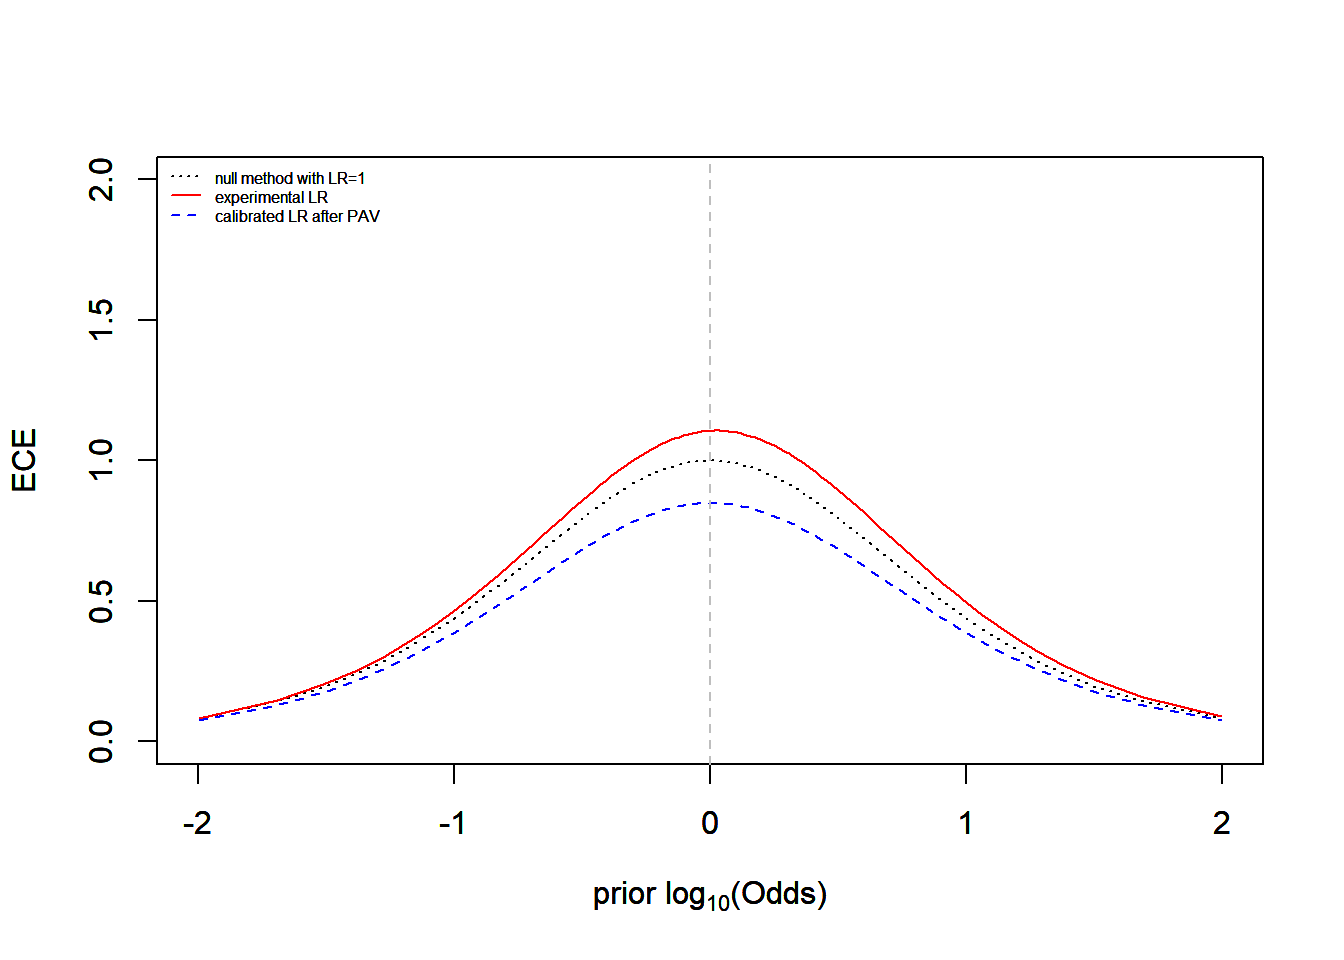
\includegraphics[scale=0.8]{InkECE1.png}
        \caption*{墨迹1的ECE图}
    \end{figure}
    \begin{figure}[H]
        \centering
        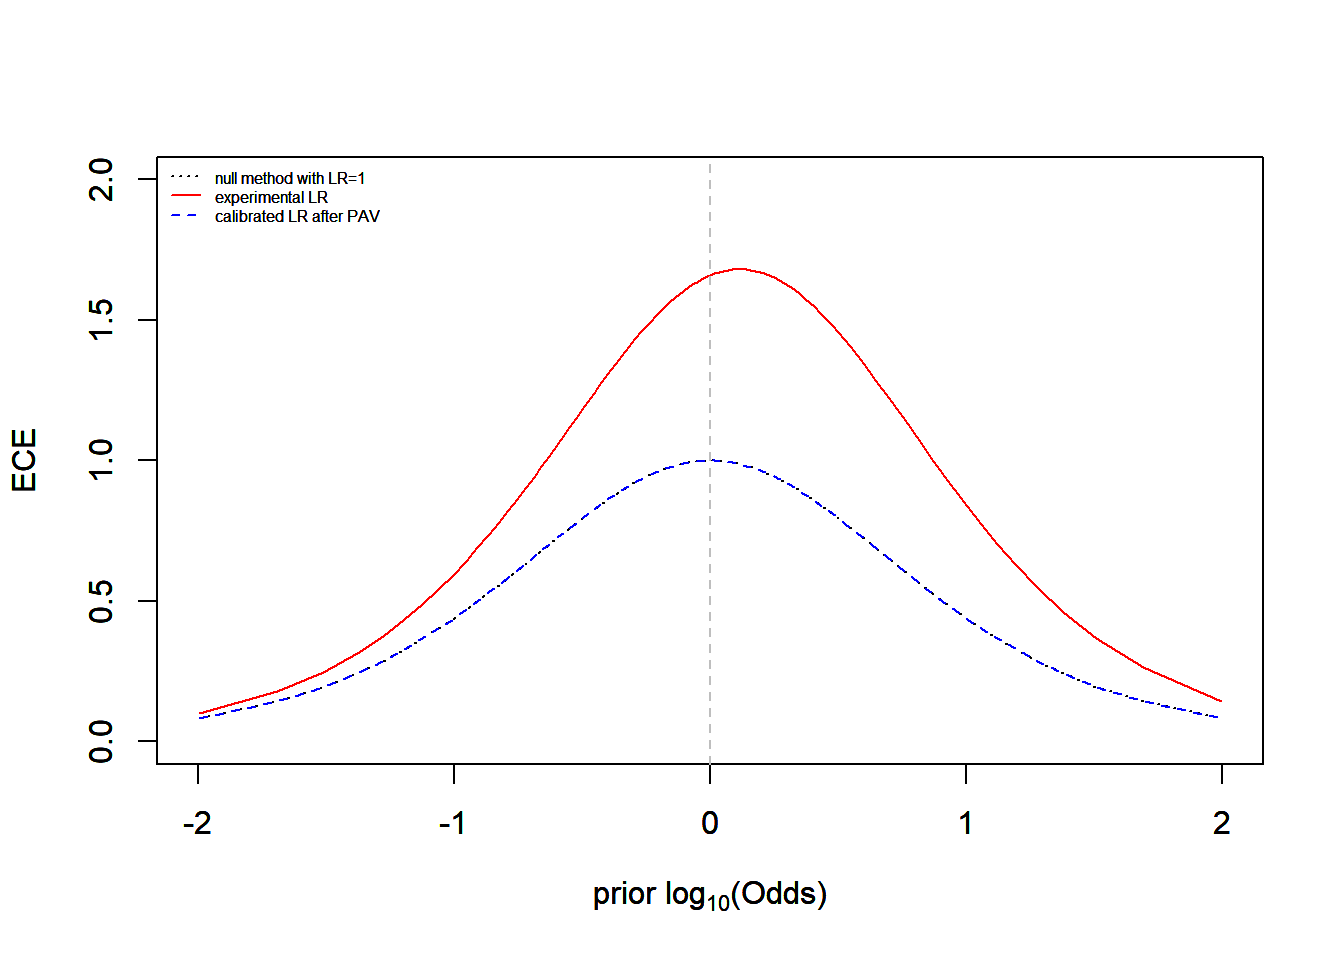
\includegraphics[scale=0.8]{InkECE2.png}
        \caption*{墨迹2的ECE图}
    \end{figure}
\end{document}